\chapter{Semantic Connection}

\section{Advantages of semantic information}

\begin{figure}[h]
\centering
%self
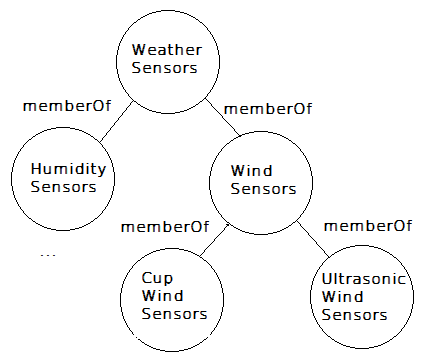
\includegraphics[width=0.6\textwidth]{figures/semws.png}
\caption{Using triples in the example\label{fig:semws}}
\end{figure}

In a cyberphisical system stored in an SOS every sensor has a name and a type. These are identifiers that correspond to a sensor and there may be other descriptors that are not informative for human reader. Sensors can be called on different names like Anemometer, Wind instrument, wind meter that means the same, measures the speed of the wind. Filtering for name is not a good approach for filtering the information. To make monitoring simpler. A semantic information is needed that organizes the data in a way that is convenient for the human reader to read. The sensors should be separated into different groups and subgroups and these groups should have an easily distinguishable name. Such groups can be Phyisical sensors -> Weather Sensors -> Wind sensors -> Wind speed sensors. This information yet can not be stored on the SOS server a separate ontology database shall be created. 
The usual way to store such information is in an ontology. 
The most widespread ontology storage standards are the RDF databases.

\section{Resource Definition Framework}

The RDF standard\cite{rdf} is created to be used with the Semantic Web approach to expand web pages with additional meanings that makes machines capable of understanding and reasoning about a web page. For example a web store can be easily understand by a customer: it has items, prices, shipping information, etc. However, for machines without saying explicitly that the value in one field is the price in USD it can be easily confused by the dimensions or the performance. Although nowadays these problems can be solved by machine learning, it is still a resource intensive process. To solve this problem an XML based standard has been introduced. This is done by using triples. 

The triple describes \textit{which} page or entity is connected on \textit{what} property to \textit{which} other page or entity. These triples are separate three unique values. 
Each value could have another triple describing it. 
Each unique identifier is a fully qualified domain name and a hash tag and a unique name, like a URL with an anchor on a web page. The first part is called the subject, the second one is the predicate, the third one is the object. 
The original idea behind the fully qualified domain name is that the approach was designed to give semantic meanings for web pages. 
Pages could refer to each other and give a global knowledge that is understandable by computers too. 

Such recursive data can be represented in graph databases, where reasoning is only walking in the database. There are graph databases to store these triples and also dedicated RDF databases. The standard way to query RDF databases is using SPARQL queries. Although RDF can represent data and connections it can not describe the rules how the reasoning, the walks in the graph should be done. These are represented by OWL or SWRL which are an extension to the RDF. However, most RDF databases also support such rules.

\begin{figure}[h]
\centering
%http://blog.52north.org/2014/02/21/sos-js/
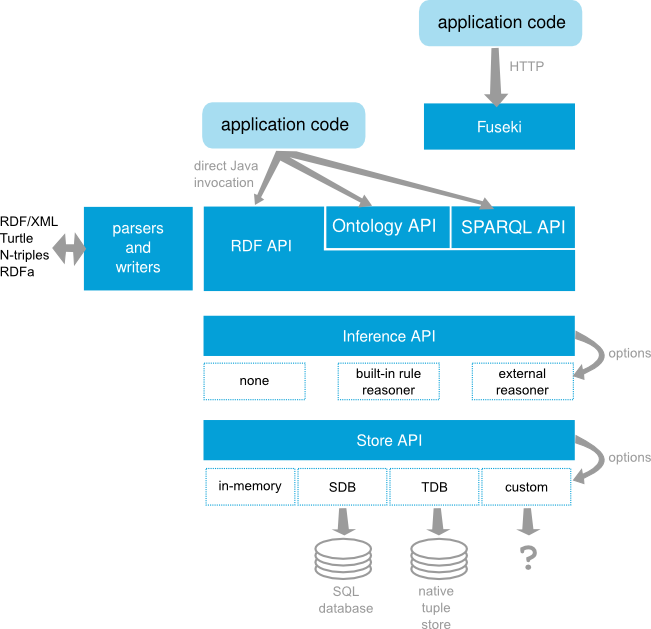
\includegraphics[width=0.6\textwidth]{figures/jena-architecture.png}
\caption{Architecture of Apache Jena\label{fig:jena}}
\end{figure}


\section{Some open source RDF databases} 

Apache Jena is an open source RDF datastore supported by the Apache foundation. It is written in Java\cite{jena}. It has many interfaces and supports many database backends. It can be used with in memory databases, SQL RDBs, triplestores. There is a built-in reasoner in the datastore, however it can be changed to other external reasoners too. The architecture of the software is shown on figure \ref{fig:jena}.

OpenRDF Sesame is another tool for storing RDF triples. It is also written in Java. It has three different interfaces for communication: the SAIL API, the RIO interface and an HTTP client. The whole application runs from a Java container like Tomcat.

Apache Foundation also supports another RDF and Graph related project called Apache Marmotta. It was started in 2012. It supports a wide range of datastore engines from in memory databases through SQL servers to large distributed column bases stores like Apache Cassandra. 

There is an out of the box tool that contains better reasoners, has a basic GUI and accepts different data types. This is Stardog database. It is a commercial application. However, it has a community version with a few restrictions. The software is written in Java and run from a web container, like Tomcat. It supports many interfaces such as HTTP and SNARL, it has a built in reasoner with integrated constraint validation. Connectors for different programming languages are ready to use. It can be easily queried using SPARQL. It has support for OWL 2 rules. Because it is an easy to use, out of the box tool this database  is used in the sample application.

\begin{figure}[h]
\centering
%http://openrdf.callimachus.net/sesame/2.7/docs/articles/figures/sesame-components.png
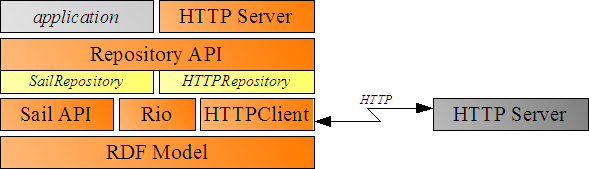
\includegraphics[width=0.6\textwidth]{figures/sesame-components.png}
\caption{Components of Sesame\label{fig:sesame}}
\end{figure}

\section{SPARQL for the queries}

To retrieve the necessary metadata the SPARQL query language is used in the RDF databases. These queries are less human readable than standard SQL queries, although they look similar. The language builds on the subject-predicate-object triples. In a result all matching data is responded. 
A SPARQL query usually has a selection part and a filtering part. 
The selection part shows which parameters should be returned. The filtering part shows which attributes are defined and it can also apply built-in functions for example language selection. 
Multiple conditions are separated with dots or commas. Commas are only used when the condition is about the same object as the previous query.  A sample SPARQL query is shown in listing \ref{lst:sparql}.

\begin{lstlisting}[caption={Sample SPARQL that queries all filterable objects\label{lst:sparql}}]
select ?s { <uri#filterable> <uri#subPropertyOf> ?s }
\end{lstlisting}

With such technology the triples can be stored and retrieved. However, the ontology behind the measurement is still missing. For that there is a standard ontology for sensors maintained by the Semantic Sensor Network Incubator Group. The underlying system which will be introduced in the next chapter is using this ontology in a somewhat customized way\cite{g2d2}.  The ontology is described in the next section.

\section{The Semantic Sensor Network Ontology}

The Semantic Sensor Network Incubator Group is a W3C incubator project. These projects are ran for one year to work on an area, this project ran from March of 2009 to September of 2010. It has developed an ontology for the semantic annotation of the Sensor Web Enablement standard. The ontology is available at http://www.w3.org/2005/Incubator/ssn/ssnx/ssn website, and it is conceptually organized into 10 modules. This is only a conceptual representation, the implementation consists of 41 concepts and 39 object properties. It is built upon a lightweight ontology, the  DOLCE-UltraLite. This underlying ontology helps the the new one to connect with other semantic databases and to have a better understanding of the concepts behind the properties. 
The ontology can be viewed from four different perspectives:
\begin{itemize}
\item A sensor perspective with focus on what and how it senses and what it sensed.
\item An observation perspective which focuses on the observation and its environment.
\item A system perspective in focus on the network itself and the deployment.
\item A feature and property perspective which focuses on the physical properties and the subject of the observation. 
\end{itemize}